% Drawing 83/10-4 -- folder 83, batch 10, archive page 200 (PDF page 201).
% Transcription: second cube, arêtes $b$, $b'$ renforcées, faces $f$, $f'$, étiquettes $t''$, $a'$.
% Kind: cube with reinforced edges. Method 2 (schematic redraw from the facsimile). Status: partial.
% Notes: Bbox re-centred on the second cube. Where his strokes meet, they meet at one computed corner: A (top left: the top left edge, the left vertical and the dotted front top edge), B (front top right: the dotted edge, the heavy edge b and the front right vertical), C (top right: the heavy edge b and the top back edge), E (bottom left: the left vertical and the heavy bottom edge b'). Elsewhere the strokes stop short as on the page and are drawn so: the top left edge and the top back edge do not reach each other (the back top corner is not drawn), the back right vertical stops below C and above the bottom, the front right vertical and the heavy edge b' stop short of the bottom front corner, and the bottom right edge (drawn with heavy dots) stops short at both ends. Also drawn: the hidden middle vertical, the oblique inner stroke at the lower left and the short stroke at the lower right, two curved arrows (one hooked down on the front face, one on the right face). Labels at \small: f (top), f' (right face), b on the heavy top edge (overinked blot there), b' over the heavy bottom edge, t'' at the bottom of the front face. Still differs: the small marks strung along the two dotted edges (letters or ticks, not legible) are left out; the mark at the lower left of the front face, read here as a' after the transcription, is not legible on the crop and is placed by position; the curved stroke right of t'' (part of a label?) is left out. Redrawn 2026-11-09 (issue 128): to check again. Overlay check 2026-11-13 (issue 147, Claude claude-opus-5-5): the redraw, rasterised by the skill's previewer (not compiled: no TeX in the session), laid over the 300 dpi colour crop of the scan (250 ppi). The cube's edges, the heavy edges b and b' and the dotted strokes lie on their ink to within 1 to 2 units. Still differs, as said above: the small marks strung along the two dotted edges are not legible and are left out, the mark read a' is placed by position, and the curved stroke right of t'' is left out.
% Coordinates: 1 unit = 1 mm = 1/100 of the crop width (bbox in page fractions: [0.12, 0.38, 0.33, 0.52]).
% Redrawn by Claude (claude-opus-5-5), issue #73, 2026-11-09; not checked by a human; not compiled (no TeX in the session).
% Checked by Claude (claude-opus-5-5) 2026-11-13 (issue #147): overlaid on the 300 dpi colour facsimile; not compiled (no TeX in the session). Status: partial.
% Rights: reproduces part of the work -- behind RENDER_TRANSCRIPTS, never published by itself.
\documentclass[tikz,border=3pt]{standalone}
\usepackage{amsmath,amssymb}
\usetikzlibrary{patterns,arrows.meta}
\tikzset{pencil/.style={black!45}, struck/.style={black!35}, mark/.style={circle,draw,inner sep=1.3pt}, pt/.style={circle,fill,inner sep=0.9pt}, opt/.style={circle,draw,fill=white,inner sep=1.1pt}}
\begin{document}
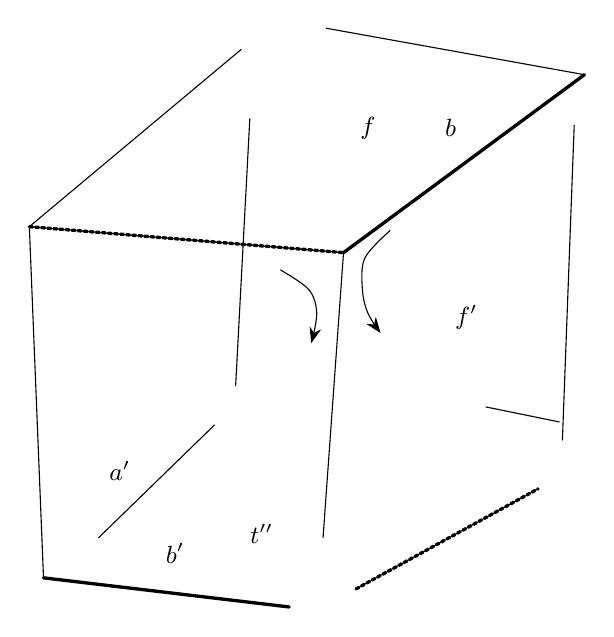
\begin{tikzpicture}[x=1mm,y=1mm,line cap=round,line join=round,font=\scriptsize]
\draw (25,-37.5) -- (51.9,-15);
\draw (62.7,-12.3) -- (95.5,-18.2);
\draw[very thick] (64.9,-40.8) -- (95.5,-18.2);
\draw (25,-37.5) -- (26.8,-82.1);
\draw[densely dotted,very thick] (25,-37.5) -- (64.9,-40.8);
\draw (64.9,-40.8) -- (62.3,-77);
\draw (94.2,-24.6) -- (92.7,-64.6);
\draw[very thick] (26.8,-82.1) -- (58,-85.8);
\draw[densely dotted,very thick] (66.5,-83.5) -- (89.6,-70.8);
\draw (53,-23.8) -- (51.2,-57.7);
\draw (33.8,-77) -- (48.5,-62.7);
\draw (83,-60.4) -- (92.3,-62.3);
\draw[-{Stealth[length=2mm]}] plot[smooth, tension=0.55] coordinates {(56.9,-43) (60.5,-45.5) (61.5,-48.5) (60.8,-52.3)};
\draw[-{Stealth[length=2mm]}] plot[smooth, tension=0.55] coordinates {(70.8,-38) (67.6,-41.5) (67.3,-45.5) (68,-48.5) (69.6,-51)};
\node[inner sep=1pt] at (68,-25) {\small $f$};
\node[inner sep=1pt] at (80.5,-49) {\small $f'$};
\node[inner sep=1pt] at (78.5,-25) {\small $b$};
\node[inner sep=1pt] at (43.5,-79) {\small $b'$};
\node[inner sep=1pt] at (54.5,-76.5) {\small $t''$};
\node[inner sep=1pt] at (36.5,-68.5) {\small $a'$};
\end{tikzpicture}
\end{document}
